\documentclass[a4paper]{article}

\usepackage[english]{babel}
\usepackage[utf8x]{inputenc}
\usepackage{amsmath}
\usepackage{amsthm}
\usepackage{amssymb}
\usepackage{enumitem}
\usepackage{graphicx}
\usepackage{caption} %prereq for subcaption
\usepackage{subcaption}  %ALLOWS SUBFIGURES
%\usepackage[colorinlistoftodos]{todonotes}
%\usepackage{tikz}
%\usepackage{algorithm,algpseudocode}

%Theorems
\newtheorem{thrm}{Theorem}
\newtheorem{lemma}[thrm]{Lemma}
\newtheorem{prop}[thrm]{Proposition}
\newtheorem{remark}[thrm]{Remark}

\theoremstyle{definition}
\newtheorem*{defi}{Definition}

%text
\newcommand{\for}{\text{ for }}

%math fonts
\newcommand{\scr}[1]{\mathcal{#1}}
\newcommand{\Z}{\mathbb{Z}}
\newcommand{\F}{\mathbb{F}}
\newcommand{\R}{\mathbb{R}}
\newcommand{\N}{\mathbb{N}}
\newcommand{\Q}{\mathbb{Q}}

%LinAlg
\newcommand{\tr}{\operatorname{tr}}

%AdvAlg
\newcommand{\opt}{\operatorname{OPT}}
\newcommand{\alg}{\operatorname{ALG}}
\newcommand{\LB}{\operatorname{LB}}


%basic probability
\DeclareMathOperator*{\E}{\mathbb{E}}
\DeclareMathOperator{\Var}{Var} 
\DeclareMathOperator{\Covar}{Covar} 
\DeclareMathOperator{\pr}{\mathbb{P}}

%Distributiondefi
\newcommand{\poi}{\ensuremath{\mathsf{Poi}}}
\newcommand{\bin}{\ensuremath{\mathsf{Bin}}}
\newcommand{\be}{\ensuremath{\mathsf{Be}}}
\newcommand{\mult}{\ensuremath{\mathsf{Mult}}}

%braces etc
\newcommand{\braces}[1]{\left\lbrace {#1} \right\rbrace}
\newcommand{\sqbr}[1]{\left\lbrack {#1} \right\rbrack }
\newcommand{\abs}[1]{\left\lvert {#1} \right\rvert }
\newcommand{\ceil}[1]{\left\lceil{ #1 } \right\rceil}
\newcommand{\floor}[1]{\left \lfloor {#1}\right\rfloor}
\newcommand{\parens}[1]{\left( {#1} \right)}


%invariant enviroment
\newenvironment{invariants}{%
  \refstepcounter{thrm}%
  \paragraph{Invariants~\theprop}%
  \renewcommand*{\theenumi}{\theprop\,(I\arabic{enumi})}%
  \renewcommand*{\labelenumi}{(I\arabic{enumi})}%
  \enumerate
}{%
  \endenumerate
}

%utility
\newcommand{\id}{\mathrm{Id}}
\newcommand{\inv}[1]{{#1}^{-1}}
\newcommand{\half}{\frac{1}{2}}
\newcommand{\third}{\frac{1}{3}}
\newcommand{\goes}{\rightarrow 	}
\newcommand{\ifftext}{if and only if }

%vectors and matrices
\newcommand{\zerov}{\vec{0}}
\newcommand{\onev}{\vec{1}}

\newcommand{\twovec}[2]{\parens{ \begin{array}{c}#1 \\ #2\end{array} }}
\newcommand{\threevec}[3]{\parens{ \begin{array}{c}#1 \\ #2\\#3 \end{array} }}
\newcommand{\fourvec}[4]{\parens{ \begin{array}{c}#1 \\ #2\\#3\\#4 \end{array} }}
\newcommand{\twomatrix}[4]{\parens{\begin{array}{cc}#1 & #2 \\ #3 & #4 \end{array}  }}
\newcommand{\twodiagmatrix}[2]{\parens{\begin{array}{cc}#1 & 0 \\ 0 & #2 \end{array}  }}


\title{The correctness of Fusy's algorithm}
\author{Sander Beekhuis, nr: 0972717}
\date{\today} %\today%

\begin{document}
\maketitle

\newcommand{\C}{\scr C}
\renewcommand{\P}{\scr{P}}


The algorithm will always maintain the following three invariants

\begin{invariants}
  \itemsep=-4pt

\item \label{i:1} The cycle $\C$ contains the two edges $S_rS_b$ and $S_rN_b$.
\item \label{i:2}No edge in the interior of $\C$ connects two vertices in $\C\setminus{S_r}$
\item \label{i:last} All inner edges of $T$ outside of $\C$ are colored and oriented in such that the innnervertex condition holds. %TODO what is the inner vertex condition
\end{invariants}

A cycle satisfying these three invariants will have the same general shape as in figure \ref{fig:invCycle}. We note that the cycle has at least $4$ vertices because otherwise a seperating triangle is created. 

\begin{figure}[h!]
\centering
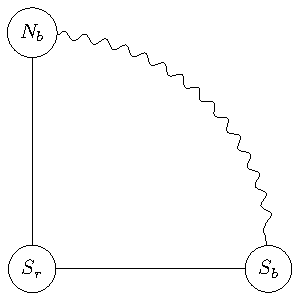
\includegraphics{img/algo/invCycle}

\caption{An example of a cycle $\C$ satisfying the invariants 
    \label{fig:invCycle }}
\end{figure}

It is also nice to note that the union of the cycle and it's interior form a triangulation of the $n$-gon since it is a induced subgraph of a triangulation of the $4$-gon.

If we remove $S_r$ from $\C$ we are left with a path from $N_b$ to $S_b$. We can then order nodes of the path by their distance (over the path)  to $S_b$. Thus $N_b$ is maximal while $S_R$ is minimal. For any two vertices $v > v'$ in this path we will denote by $[v, v']$ the subpath from $v$ to $v'$.

\begin{defi}[internal path]
We call a path $\P$ an internal path of $\C$ if  all its edges are in the interior of $C$ and it connects two distinct vertices of $\C$ 
\end{defi}

%TODO define \C_\P

\begin{defi}[eligible path]
We call an internal path $\P$ from $v$ to $v'$ eligible if 
\begin{enumerate}
 \renewcommand*{\labelenumi}{(E\arabic{enumi})}%
 \renewcommand*{\theenumi}{(E\arabic{enumi})}%


\item Neither $v$ or $v'$ is $S_r$ \label{e:notSr}
\item The paths $\P$ and $[v,v']$ both have at least 3 vertices \footnote{that is, they have an interior vertex} \label{e:internalVertices}
\item Each edge in the interior to $\C_\P$ connects a vertex of $\P\setminus{v,v'}$ and $[v,v']\setminus{v,v'}$. In particular $\C_\P$ is a non-separating cycle.
\label{e:crossingedge}
\item The cycle $\C'$ obtained by replacing $[v,v']$ by $\P$ in $\C$ has no interior edge connecting the two vertices of $C\setminus{S_r}$.
\label{e:noIntEdgeInC'}
\end{enumerate}
\end{defi}

\section{If the invariants are satisfied there always is an \emph{eligible} internal path}

We will show the following proposition.

\begin{prop}
When the algorithm's invariant (\ref{i:1} - \ref{i:last}) are satisfied and the cycle $\C$ is separating then there exist a \emph{eligible} internal path.
\end{prop}

\begin{proof}
We will first show that there always exists an internal path $\P$. We will then show that a internal path can be found that satisfies conditions $(E1) - (E4)$.

In the proof we will often use that a 

Let us first note that if the cycle $C$ is separating (i.e has a non-empty interior), there is at least one interior vertex $v$. Since the triangulation of a $n$-gon is $2$-connected there are two ways to go from $v$ to (say) $S_r$. Hence there is an internal path $\P_0$.

If this path does not satisfy \ref{e:notSr} we can use the following construction. The other vertex where $P_0$ intersects $\C$ is not $S_r$. Let us call this vertex $x$ and it's neighbour on the path $y$. The vertex $x$ might be $N_b$ or $S_b$ but can't be both, hence it has at least one neighbour $z$ on the cycle that is not $S_r$. Because the triangulation of a $n$-gon is internally maximally planar we have that $yz$ is an edge. Now $xyz$ is an internal path satisfying \ref{e:notSr}. See also figure \ref{fig:E1}, here we made a choice on which side of $y$ the vertex $z$ lies, but this choice can be made without losing generality.

Hence we have now constructed, or already had, a path that satisfies \ref{e:notSr}. Let us for the remainder of the proof denote this path by $\P_1$.


If $\P_1$ satisfies (E2) we set $\P_2 = \P_1$ otherwise we will create a path that satisfies (E1) and (E2). 
If the path $\P_1$ does not satisfy $(E2)$ \footnote{which will be the case if the above construction has been used} then there are two possibilities  a) $\P_1$ does not have interior vertices and/or b) $[v,v']$ does not have interior vertices. If a) would be true the existence of $P_0$ would contradict Invariant \ref{i:2}. Hence the only problem can be that $b)$ occurs. 

If $v=N_b$ and $v'=S_b$ we have found a separating triangle given by $S_rN_bS_b$ \footnote{this is the cycle $\C$ which is separating} in original graph. Hence at least one of $v$ or $v'$ is not $N_b$ or $S_b$. If we call this vertex $x$ its neighbour on the path $y$ and it's neighbour outside $[v,v']$ $z$. We see that by the interior of $\C$ being maximally planar $yz$ must be an edge. If we now adapt $P_1$ by replacing $yx$ by $yz$ we have made $[v,v']$ one vertex longer and hence created a path satisfying \ref{e:internalVertices}. In figure \ref{fig:E2} we show this procedure in two cases. Executing this procedure does not change that $S_r$ is not one of the endpoints of the path. Hence we have now created a path $\P_2$ that satisfies \ref{e:notSr} and \ref{e:internalVertices}.

\begin{figure}
    \centering
    \begin{subfigure}[b]{0.45\textwidth}
        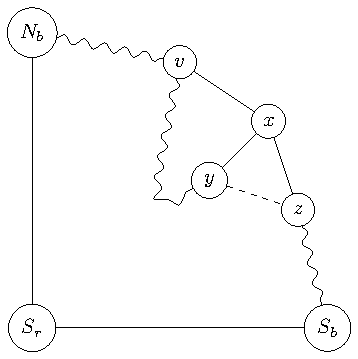
\includegraphics[width=\textwidth]{img/algo/E2general}
        \caption{The general case. Note that $x=v'$.}
    \end{subfigure}
    ~ 
    \begin{subfigure}[b]{0.45\textwidth}
        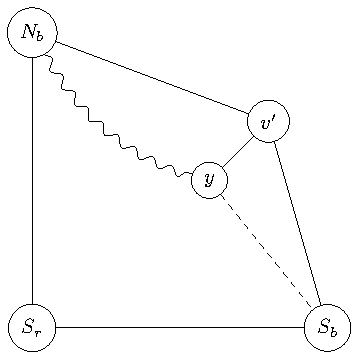
\includegraphics[width=\textwidth]{img/algo/E2spec}
        \caption{A specific case. Note now that $N_b=v, v'=x$ and $S_b=z$}
    \end{subfigure}

    \caption{Creating a path satisfying \ref{e:internalVertices}. The dotted line is the edge we take in the new path $\P_2$}\label{fig:E2}
\end{figure}

\newcommand{\intvv}{\ensuremath{[v,v']\setminus{v,v'}}}
\newcommand{\intP}{\ensuremath{\P\setminus{v,v'}}}

If $\P_2$ satisfies $(E3)$, we take $\P_3 = \P_2$. Otherwise we will remedy the defect. We separate five different cases of offending edges. All of the five cases will be easy to remedy giving a path $\P'_2$ still satisfying \ref{e:notSr} and \ref{e:internalVertices} such that $\C_{\P'_2}$ is strictly contained in $\C_{\P_2}$ %Q what is the right version of smaller here?
\begin{enumerate}
 \renewcommand*{\labelenumi}{\alph{enumi})}%
 \renewcommand*{\theenumi}{\alph{enumi})}%
 \item edges from \intvv to $\intvv$
 \item edges from $\intP$ to $\intP$
 \item edges incident to $v$ or $v$ and some other vertex on $\C_{\P_2}$
 \item edges from $[v,v']$ to some internal vertex 
 \item edges from $\intP$ to some internal vertex
\end{enumerate}

The existence of an edge as in a) is forbidden by Invariant \ref{i:2}. If b) occurs we can simply shortcut our original path $\P_2$ with this edge. If c) occurs this edge can't go to another vertex in $[v,v']$ since that would offend Invariant \ref{i:2}. Hence they go to a vertex in $\P_2$ and we can shortcut the path as in b).

If d) occurs we simply make a new path and if e) occurs we take a slightly adapted interior path. See figures

%TODO pictures

Since all of the moves shrink $\C_{\P_2}$ while keeping \ref{e:notSr} and \ref{e:internalVertices} intact and we can't idenfinitly shrink this means at a certain point no more moves are availble. Since every offending edges allows a move this means that there are no more offending edges. Hence this version of $\P'_2$ satisfies \ref{e:crossingedge}. For the final step of the proof we take $\P_3 = \P'_2$.

%TODO formulate repetition argument nicly

Suppose that $\P_3$ does not satisfy \ref{e:noIntEdgeInC'}. Then we can just take the would be interior edge and take this for a nwe path. This is again a finite procedure reducing the sum of $|\P_3| -|[v,v']|$. In the end we have a path satisfying \ref{e:notSr} - \ref{e:noIntEdgeInC'}.

%TODO picturse, why dont we lose E1-E3


\end{proof}

\begin{figure}[h!]
\centering
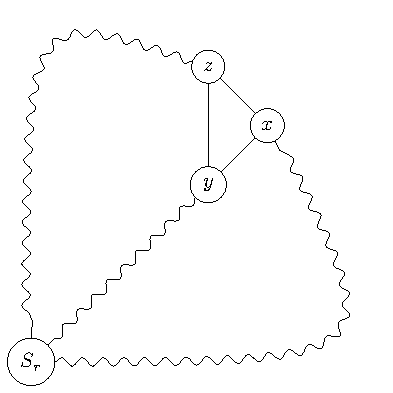
\includegraphics[]{img/algo/E1}
\caption{Constructing a path satisfying \ref{e:notSr} \label{fig:E1}}
\end{figure}

\end{document}
